\pagestyle{empty}
\cleardoublepage
\pagestyle{fancy}

\chapter{Geração de Malhas}\label{cap3}

Nesse capítulo, serão apresentadas as técnicas de geração de malhas bidimensionais mais conhecidas atualmente. Existem diversos algoritmos para geração de malhas, porém todos eles podem ser enquadrados em três categorias que iremmos descrever a seguir:

\begin{itemize}
  \item Avanço de fronteira: a malha deve ser gerada a partir da borda da região;

  \item Delaunay: procura-se maximizar o menor ângulo dos triângulos gerados para um dado conjunto de pontos;

  \item Arbitrária: para todos os outros tipos de malhas;
\end{itemize}

\section{Avanço de fronteira}

Este é um dos métodos mais populares de geração de malhas e consiste em criar os elementos no interior do domínio progressivamente a partir de um contorno especificando da região a ser preenchida (fig.~\ref{fig:imagem7}a). Este contorno é chamado de fronteira inicial ou borda, os elementos são gerados a partir dessa fronteira dada como entrada. Uma fronteira bidimensional é formada por um conjunto de arestas.

À medida em que o algoritmo progride, a fronteira avança em direção ao interior, sempre removendo ou adicionando elementos de fronteira até que todo o domínio seja preenchido. O algoritmo chega ao fim quando não há mais fronteira, ou seja, o domínio foi totalmente triangularizado. 

Pode ocorrer do algoritmo não conseguir mais gerar elementos para uma determinada fronteira, isso indica que o algoritmo falhou. O caso de falha ocorre quando todos os possíveis elementos a serem criados se sobrepõe um elemento já existente. Por isso a importância de verificar se um elemento criado não sobrepõe um elemento já existente. Os casos de falha geralmente acontecem em modelos tridimensionais.

Para gerar os novos triângulo no interior do domínio é necessário criar novo pontos que não pertencem à entrada, em geral é utilizados os pontos de Steiner para isso.

Enquanto houver arestas na fronteira um algoritmo nessa categoria irá proceded da seguinte forma no caso 2D (fig.~\ref{fig:imagem7}):
 
 \begin{enumerate}
\item{ Remova uma aresta da fronteira, a aresta base (fig.~\ref{fig:imagem7}b)}
\item{ Encontre um ponto ideal para a formação de um novo triângulo com a aresta base (fig.~\ref{fig:imagem7}c),}
\item{ Crie uma região de busca em torno desse ponto ideal (fig.~\ref{fig:imagem7}d),}
\item{ Selecione o ponto dentro dessa região de busca cujo triângulo (entre esse ponto e a aresta base) seja válido e seja o de melhor qualidade,}
\item{ Forme o novo triângulo com o ponto selecionado e adicione-o à malha (fig.~\ref{fig:imagem7}e),}
\item{ Atualize a fronteira, inserindo as arestas que foram criadas, e removendo as arestas que já existiam,}
\item{ Se existir aresta na fronteira, volte para o passo 1.}
\end{enumerate}

 \begin{figure}[htbp]
     \centering
     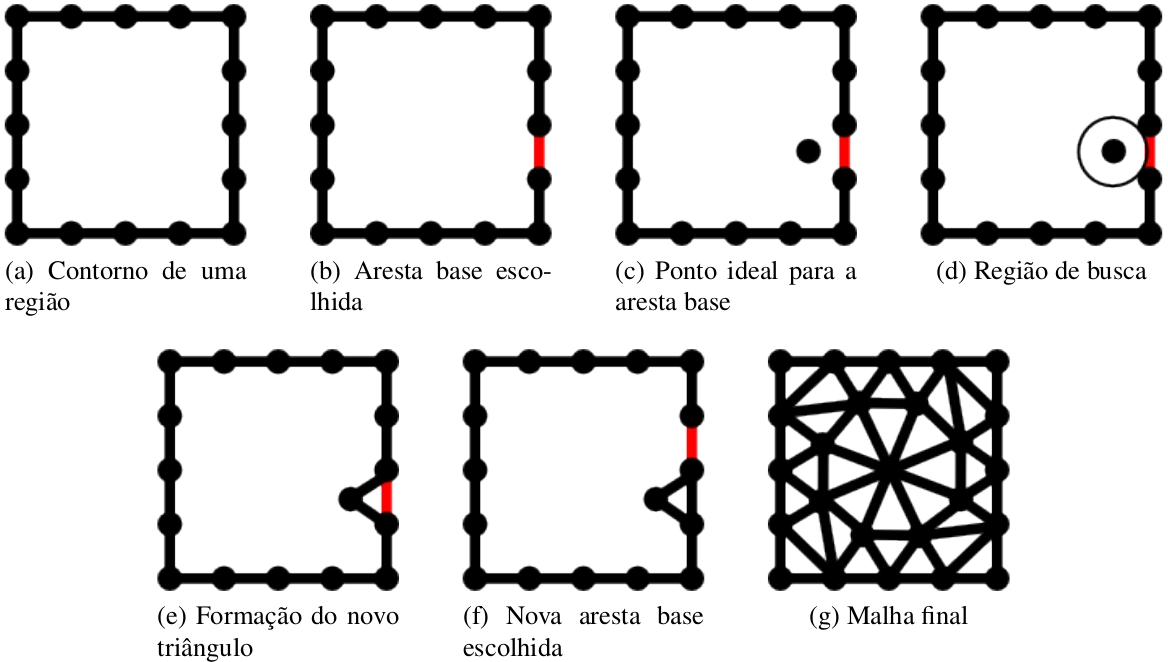
\includegraphics[width=1\textwidth]{imagem7}
     \caption{Avanço de fronteira. \cite{bib:Freitas10}} 
     \label{fig:imagem7}
 \end{figure}

 Pelo fato da fronteira ser sempre respeitada, os algoritmos de avanço de fronteira têm facilidade em tratar regiões descontínuas, ou por conterem buracos, ou por serem regiões separadas. Como os elementos mais próximos da borda são gerados primeiro, eles irão ter em geral uma boa qualidade. A boa qualidade da malha gerada provem estabilidade e precisão na aplicação de métodos numéricos (como os métodos dos elementos finitos).

Porém, nem sempre todos os elementos gerados terão boa qualidade. Ao contrário dos elementos mais próximos da borda, os elementos mais internos à malha nem sempre teão boa qualidade devido à região torna-se menor a medida que a fronteira avança. Geralmente uma técnica de suavização ou otimização é aplicada na malha resultante do algoritmo para tratar esses casos.

\section{Delaunay}

Essa é um técnica bastante conhecida na área de geração de malhas, a origem do nome vem do matemático russo Boris Delaunay. A entrada para esse problema é um conjunto de pontos, nesse caso não é utilizado os pontos de Steiner para formar os triângulos.

O critério de Delaunay para a formação dos triângulos é que não exista nenhum outro ponto dentro do círculo que passa pelos três pontos desse triângulo, esse critério pode ser chamado também de “esfera vazia” (o circuncírculo desse triângulo, Figura~\ref{fig:imagem8}). O critério de Delaunay em si não se constitui num método de geração de malhas, mas é uma forma de saber onde os pontos devem estar localizados no espaço.

 \begin{figure}[htbp]
     \centering
     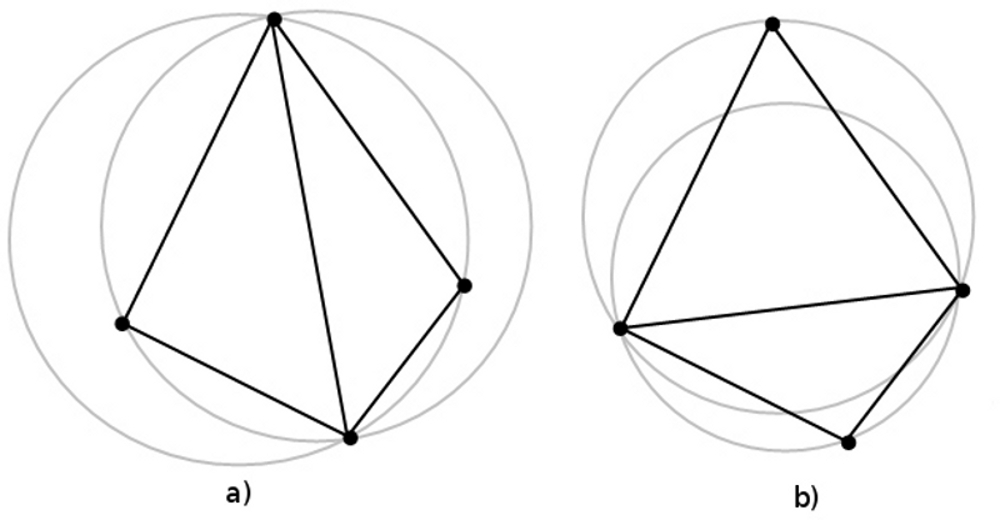
\includegraphics[width=1\textwidth]{imagem8}
     \caption{a) critério de Delaunay falhando para os dois triângulos. b) Triangulação valida respeitando o critério de Delaunay.} 
     \label{fig:imagem8}
 \end{figure}

A malha gerada por Delaunay visa maximizar os ângulos internos dos triângulos gerados. Ou seja, dada uma aresta da triangulação de Delaunay, o ponto que forma o maior ângulo com essa aresta é o ponto que formará um triângulo de Delaunay com os outros 2 pontos desta aresta.

Existem dois tipos de algoritmos de Delaunay. No primeiro tipo, encontra-se uma aresta que faz parte da triangulação, em geral é selecionada uma aresta que pertence ao fecho convexo como primeira aresta. A partir da primeira aresta é encontrado o ponto que formará um triângulo de Delaunay. Assim, com as novas arestas, encontra-se novos triângulos, em um algoritmo parecido com o de avanço de fronteira. No segundo tipo, a entrada é uma malha triangular não necessáriamente de Delaunay e se modifica essa malha (de apenas um subconjunto de pontos da entrada) pré-existente (Figura~\ref{fig:imagem9}).

 \begin{figure}[htbp]
     \centering
     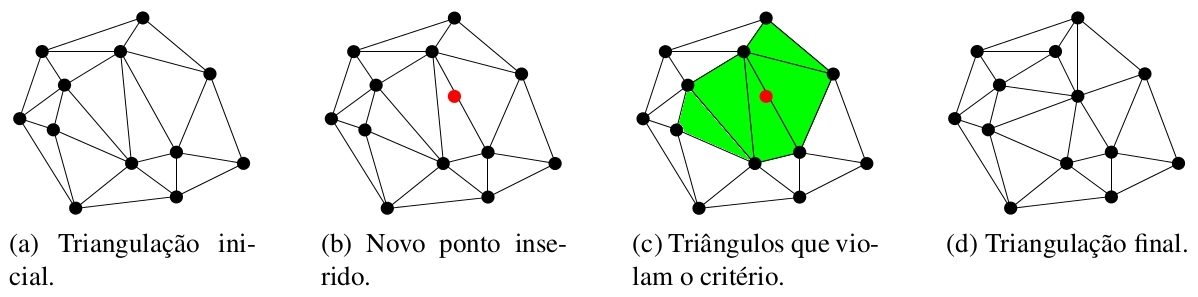
\includegraphics[width=1\textwidth]{imagem9}
     \caption{Triangulação por inserção de pontos. \cite{bib:Freitas10}} 
     \label{fig:imagem9}
 \end{figure}

 Dependendo da disposição dos pontos da entrada a triangulação final pode não têr boa qualidade, gerando instabilidade em métodos numéricos. Uma alternativa para melhorar essa malha é fazer refinamentos e otimizações, que fazem uso de pontos de Steiner, são utilizados para se melhorar a qualidade da malha.

\section{Arbitrária}

Vamos definir as chamadas malhas arbitrárias aquelas que não se enquadrarem nem como avanço de fronteira nem como Delaunay. Essas malhas em geral são geradas por algoritmos de varredura ou algum outro método. 

Outro uso que essas malhas possuem é na demonstrações de teoremas sobre malhas. O problema de ordenação de pontos pode ser reduzido ao problema de geração de malhas bidimensionais \cite{bib:CarvalhoFigueiredo91}. Prova-se por redução que pode ser gerado uma malha triangular a partir do fecho convexo de um conjunto de pontos em duas dimensões numa complexidade na ordem de (n log n).
